\chapter{Background}


\section{Computer Aided Diagnostics}

Machine learning techniques have been successfully applied to computer-aided diagnosis where it by a computerized procedure provides a second objective opinion for the assistance of medical image interpretation and diagnosis \parencite{li2007}, \parencite{ni2016}. To make a CAD system samples with diagnosis i used for learning. In the case of breast cancer diagnosis a radiologist put labels on a set of mammography scans. Labels that includes the diagnosis of the scan a possibly some attributes of the scan too. These scans togeather with the labels can then be used to learn a hypothesis whether a undiagnosed sample is benign or malignant cancer \parencite{li2007}.


\section{Breast Cancer}

A study in Sweden by \textcite{tabar2001} found breast carcinoma mortality was reduced by 63\% after mammography was introduced. This clearly emphasize the benefits of screening which had resulted in a increased usage of the method to detect and diagnose breast cancer. The increasing demand for mammography image interpretation lead to a shortage of medical radiologist to perform this task and consequently non medical personnel supplement the mammography image interpretation \parencite{culpan2016}. As breast cancer still continues to be the leading cause of cancer mortality among women and more efficient diagnostics and pathology is high on demand the need of low-cost point-of-care is very much needed as stated by \textcite{martei2018}.

Fine needle aspiration (FNA) is a diagnostic tool to aspirate cell samples by sampling cells, staining them and examine under a microscope \parencite{FNA}. An example of such sample can be seen in \ref{fig:fna_nuclei}. The cell samples can be evaluated within 24 hours and the method is cost-effective and can be used as a preoperative tool for investigation of tumors. The method is also complication-free and has been widely used for the past 60 years.

\begin{figure}[ht!]
  \centering
  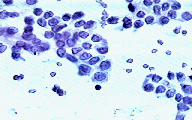
\includegraphics[]{images/fna_nuclei.png}
  \caption{A caption of a FNA sample as seen through a microscope. Image courtesy of Wisconsin University}
  \label{fig:fna_nuclei}
\end{figure}

% Image source: http://webcache.googleusercontent.com/search?q=cache:635J2rrIdWsJ:pages.cs.wisc.edu/~olvi/uwmp/cancer.html+&cd=1&hl=sv&ct=clnk&gl=se


\section{Feature Selection}

A feature is a variable that describes a data instance. A rectangular surface can be considered having two features, length and height. A rectangular volume three features, length, height and depth. More complex data instances such as a gene expression may have up to 60,000 features and such a complex feature space results in a much harder learning process. Thus one often wishes to select a subset of all available to reduce the dimensionality \parencite{guyon2003}.

The benefits of selecting a subset of all available features are manyfold, among other it facilitates data visualisation and data understanding, reduces the measurement and storage requirements and reduces training and utilisation times. In cases with thousands of features like the example with gene expressions it is essential to work with a subset of the data to produce reliable results. \parencite{guyon2003}.


\subsection{Filter methods}

Filter methods are considered as a preprocessing step. That means a filter method evaluate features before data is applied to a learning machine or even before a deciding on a classifier. The evaluation is performed by doing variable ranking by some score such as information gain. The score results in a ranking of the attributes and a subset can be selected in order of the ranking \parencite{guyon2003}.

There are both good and bad aspects of filter methods. The positive concerns that variable ranking makes filter methods very scalable and robust as the calculations only operated on as many variables as there are features and can be performed just once and tested on multiple classifiers making it very computational effective. On the other hand, a subset of features that by their own might be assessed an non informative by their own may in combination provide a lot of information to enable good learning \parencite{guyon2003}.


\subsection{Wrapper methods}

\textbf{ Pawel: Add information on each classifier. At most 1/3 of a page describing their functionality on  vary high level }

Wrapper methods differs a lot from filter methods. While filter methods evaluate the as a preprocessing independent of the classifier, wrapper does the opposite.

Wrappers utilise the learning machine of interest as a black box to score subsets of variable according to their predictive power \parencite{guyon2003}. The issue is as datasets become very large this method might be overly computational intense as finding the optimal subset is considered to be NP-hard \parencite{amaldi1998}.


\section{Related Work}

\textbf{ Pawel: Make subsections where each section coves a specific topic. This can also be extended with almost another full page.}

The application of machine learning onto breast cancer classification is a well studied one. Since machine learning proved valuable empirical results breast cancer datasets have been widely used to assess the performance of a multitude of classification strategies and methods. [Insert ref. to early paper here].

Exhaustive studies for optimal Classifiers has been made as by \parencite{ramos2012} which tested 20,000 classification configurations to evaluated their ability to correctly classify malignant cancer. The achieved a result of 0.996 under the Receiver operating characteristic (ROC) curve.
% Add which method achieved the result above

With a foundation of well performing classifiers studies investigating more fine tuned approaches building upon earlier results were being made. \textcite{akin2011} demonstrated that ensemble learning can be used in CAD to improve the performance of rotation forest classifier. Using three different dataset and 30 classifying algorithms the average accuracy improved on all datasets by nearly 3\%.

\textcite{Abdel-Ilah2017} reported further improvements on ANNs by investigating the optimal number of hidden layers and neurons for a feed forward back propagation network. The highest accuracy acheived was 98\% using 3 hidden layers and 21 neurons with three distinct transfer functions.

\textcite{akay2009} investigated the performance of classification of a SVM with a RBF kernel using feature selection, filtering by F-score. They achieved a classification accuracy of 99.51\% which accordingly was among the highest scores recorded by then (2007).

\textcite{karabulut2012} made a comparative study on the effect of feature selection on classification accuracy and found up to 15.55\% improvement on classification rates. The study used only filter algorithms for feature selection, among those were both information and Chi-square. The study applied the selected features on three classification methods, Naive Bayes, Artificial Neural Network as Multilayer Perceptron, and J48 decision tree classifier on 15 different datasets including WBCD.

Building upon this foundation of work our study seeks to complete the field by providing further investigation of unreported selection methods such as SBS and SFS and review their performance on a combination of classifiers from the previous research presented here.
